\capitulo{4}{Técnicas y herramientas}


\section{Técnicas de desarrollo}

\section{Herramientas de documentación}
\subsection{LaTex}
Se trata de un sistema de composición de textos, con el objetivo de la creación de documentos de alta calidad tipográfica.
\section{Herramientas de gestión}
\subsection{GitHub}
Se trata de una plataforma donde se pueden guardar con un sistema de control de versiones los proyectos....

 Link del repositorio: \url{https://github.com/smi0010/TFG_Herramientas_Realidad_Aumentada}

\section{Herramientas de desarrollo}
\subsection{Unity}
Unity, es un motor gráfico de desarrollo de videojuegos creado por Unity technologies, disponible para Windows,Linux y Mac OS.

Instalación.

Para Instalar el motor unity es necesario descargar Unity Hub: \url{https://store.unity.com/es/download-nuo}

Unity Hub se trata de un launcher desde el que se pueden, descargar varias versiones de Unity simultáneamente, pudiendo escoger la que mejor se acomode a las necesidades del usuario. También ofrece una serie de tutoriales para iniciarse en el desarrollo de Unity. Por ultimo ofrece un listado de los proyectos del usuario, así como a que versión pertenecen, pudiendo escoger con que versión de Unity desean ejecutarlos.

En la pestaña de installs, pulsando el botón "Add", saldrá una venta donde poder escoger la versión deseada, al pasar el siguiente paso deberemos escoger los módulos complementarios para Unity, por el momento sería necesario el de Android, para poder pasar nuestros proyectos a una aplicación Android, importante desplegar las opciones del modulo y seleccionar ambas, pues para la compilación de una aplicación es estrictamente necesario el APK de Android.

\includegraphics[scale=0.4]{Unity01}
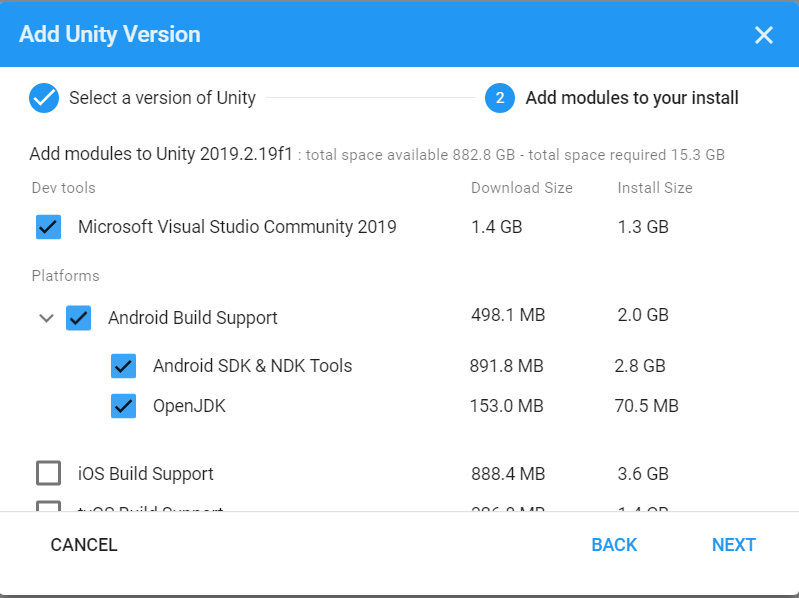
\includegraphics[scale=0.4]{unity02}

Una vez terminada la instalación ya es posible comenzar a crear proyectos. 
Para poder descargar y usar Assets desde la tienda de Unity es necesario tener una cuenta de usuario.
\subsection{title}
